\documentclass[
  11pt,
  letterpaper,
   addpoints,
   answers
  ]{exam}

% Carga el preámbulo localizado en la carpeta superior
\NeedsTeXFormat{LaTeX2e}[2023/04/30]

% Provide the name of your page, the date it was last updated, and a comment about what it's used for
\ProvidesPackage{../exercise-preamble}[2023/04/30 Prof. Cassanelli custom LaTeX style]

% \usepackage{printlen}
% \uselengthunit{in}\printlength{\textwidth}

% PACKAGES
\usepackage[dvipsnames]{xcolor}

\usepackage{graphicx}
\graphicspath{{../figures}}
\usepackage{amsmath,amsthm,amssymb,mathtools,mathrsfs}
\usepackage{commath}
\usepackage{upgreek}
\usepackage{cancel}
\usepackage{enumerate}
\usepackage[font=small]{caption}
\usepackage[normalem]{ulem}
\usepackage{steinmetz}

\usepackage[left=1.5cm, right=1.5cm, top=1cm]{geometry}

% REFERENCES AND OTHERS
\usepackage{../aas_macros}
\usepackage{natbib}
\bibpunct{(}{)}{;}{a}{}{,}

\usepackage{tikz}
\usepackage{tikz-3dplot}
\usepackage{circuitikz}
\usepackage{pgfplots}
\pgfplotsset{compat=1.15}
\usepgfplotslibrary{smithchart}
\usetikzlibrary{
  decorations.pathmorphing,
  decorations.markings,
  calc,
  patterns,
  decorations,
  angles,
  quotes,
  ext.topaths.arcthrough,
  shapes
  }

\usepackage{siunitx}
\sisetup{
    range-phrase=\text{--},
    range-units=single,
    separate-uncertainty=true,
    print-unity-mantissa=false
    }
\DeclareSIUnit{\gauss}{G}
\DeclareSIUnit{\jansky}{Jy}

\newcommand{\iu}{\mathrm{i}\mkern1mu}
\newcommand{\ju}{\mathrm{j}\mkern1mu}
\newcommand{\euler}{\mathrm{e}}
\newcommand{\exponential}[1]{\mathrm{exp}\left[#1\right]}
\newcommand{\uvec}[1]{\widehat{\mathbf{#1}}}
\newcommand{\uvecs}[1]{\boldsymbol{\widehat{#1}}}
\newcommand{\bvec}[1]{\boldsymbol{\mathcal{#1}}}

\usepackage{hyperref}
\hypersetup{
    % bookmarks=true,
    unicode=true,
    pdftoolbar=true,
    pdfmenubar=true,
    pdffitwindow=false,
    pdfstartview={FitH},
    pdftitle={EL3103},
    pdfauthor={Tomas Cassanelli},
    pdfcreator={Tomas Cassanelli},
    pdfnewwindow=true,
    colorlinks=true,
    linkcolor=Violet,
    citecolor=Violet,
    urlcolor=Violet
    }

% Exam document class
\renewcommand{\figurename}{Figura}
\renewcommand{\tablename}{Cuadro}
\pagestyle{empty}

\usepackage[spanish]{cleveref}

\crefname{question}{\protect{pregunta}}{\protect{preguntas}}
\Crefname{question}{\protect{Pregunta}}{\protect{Preguntas}}
\creflabelformat{question}{#2{#1}#3}

\renewcommand{\solutiontitle}{\noindent\textbf{Solución:}\par\noindent}
\bracketedpoints
\pointname{~puntos}

\endinput

% Paquetes locales
\usepackage{float}
\usepackage{booktabs} % para \toprule, \midrule, \bottomrule
\usepackage{xcolor} % para colores
\usepackage{bm} % para negrita en símbolos matemáticos

% Macros locales
\newcommand{\Rel}{\mathfrak{R}} % símbolo para la reluctancia
\DeclareMathOperator{\Var}{Var} % operador de varianza

\begin{document}

% Configuración del encabezado usando comandos de la clase exam
\pagestyle{headandfoot}
\extraheadheight{0.5in} % Baja el encabezado aumentando el espacio superior
\firstpageheader{\textit{Análisis de Sistemas Dinámicos y Estimación}}{}{EL3204-1}
\runningheader{\textit{Análisis de Sistemas Dinámicos y Estimación}}{}{EL3204}
\firstpagefooter{}{\thepage}{}
\runningfooter{}{\thepage}{}
\headrule % Línea debajo del encabezado

% Numeración de página
\pagenumbering{arabic}

% Portada
\begin{center}
    \vspace*{1cm}
    
    % Logo superior
    \includegraphics[width=0.5\textwidth]{../fcfm_die}
    
    \vspace{2cm}
    
    % Líneas decorativas superiores
    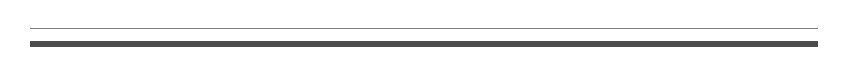
\begin{tikzpicture}
        \draw[line width=2pt, black!70] (0,0) -- (10,0);
        \draw[line width=0.5pt, black!50] (0,0.2) -- (10,0.2);
    \end{tikzpicture}
    
    \vspace{1cm}
    
    % Título principal
    {\fontsize{28}{34}\selectfont\bfseries 
    Análisis de Sistemas\\[0.3cm]
    Dinámicos y Estimación}
    
    \vspace{0.5cm}
    
    {\Large\textbf{EL3204-1}}
    
    \vspace{1cm}
    
    % Líneas decorativas inferiores
    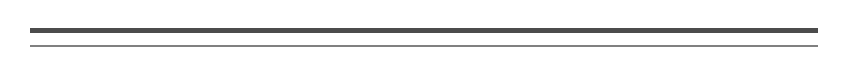
\begin{tikzpicture}
        \draw[line width=0.5pt, black!50] (0,0) -- (10,0);
        \draw[line width=2pt, black!70] (0,0.2) -- (10,0.2);
    \end{tikzpicture}
    
    \vspace{1.5cm}
    
    % Subtítulo
    {\LARGE\itshape Pauta Auxiliar 13 - Repaso Examen}
    
    \vspace{0.5cm}
    {\large Prof Marcos Orchard - Sebastian Espinoza.}\\
    {\large Prof Auxiliar Erik Sáez Aravena.}
    
    % Decoración con símbolo matemático de fondo
    \begin{tikzpicture}[remember picture, overlay]
        \node[opacity=0.5, rotate=0] at ([yshift=-8cm]current page.center) {
            \fontsize{280}{300}\selectfont\color{black!15}$\mathcal{I}(\theta)$
        };
    \end{tikzpicture}
    
    \vfill
    
\end{center}

\newpage
%----------------------------
% =========================================
% Unidad III — Estimación de Parámetros (Resumen)
% =========================================
\section*{Resumen}

Este auxiliar cubre conceptos fundamentales de la teoría de estimación de parámetros, que complementa los temas de detección vistos anteriormente. En problemas de detección, el espacio paramétrico $\Theta$ era discreto y finito, pero ahora trabajamos con un conjunto \textbf{infinito no numerable} de posibles valores para el parámetro que queremos estimar (un continuo).

\subsection*{1. Conceptos Básicos de Estimación}
Algunos conceptos importante a considerar son:
\begin{enumerate}
\item \textbf{Espacio de observación ($\mathbb{X}$):} Espacio donde la variable aleatoria $X \in \mathbb{X}$ toma valores. Para vectores aleatorios, $\mathbb{X}^n$ representa el espacio producto.

  \item  \textbf{Espacio de decisión ($\Theta$):} En estimación, es un conjunto \textbf{infinito no numerable} de valores (a diferencia de detección donde era finito). Ejemplos: $\Theta = \mathbb{R}^+$ para estimar amplitudes, $\Theta = \mathbb{R}$ para estimar medias.

\item \textbf{Familia de distribuciones paramétricas ($J_\theta$):} Conjunto de distribuciones indexadas por $\theta$:
\[
J_\theta = \{P_X(x|\theta) : \theta \in \Theta\}
\]

\item \textbf{Estimador:} Una función $\hat{\theta}(x_1, \ldots, x_n)$ que depende de las observaciones y entrega una estimación del parámetro $\theta$ asociado a la distribución $P_X(x|\theta)$.
\end{enumerate}
\subsection*{2. Propiedades de los Estimadores}
\begin{enumerate}
  \item \textbf{Estimador Insesgado:} Un estimador $\hat{\theta}(x_1, \ldots, x_n)$ es insesgado si:
\[
\mathbb{E}[\hat{\theta}(X_1, \ldots, X_n)] = \theta
\]
Es decir, en promedio el estimador entrega el valor verdadero del parámetro.

\item \textbf{Estimador Asintóticamente Insesgado:} Si el sesgo tiende a cero cuando $n \to \infty$:
\[
\lim_{n\to\infty} \mathbb{E}[\hat{\theta}(X_1, \ldots, X_n)] = \theta
\]

\item \textbf{Estimador Consistente:} Un estimador es consistente si converge en probabilidad al valor verdadero:
\[
\lim_{n\to\infty} P_X(|\hat{\theta}(X_1, \ldots, X_n) - \theta| > \epsilon) = 0 \quad \forall \epsilon > 0
\]

\item \textbf{Observación:} Mediante la desigualdad de Chebyshev, si un estimador es insesgado y su varianza tiende a cero cuando $n \to \infty$, entonces es consistente:
\[
\lim_{n\to\infty} \Var(\hat{\theta}(X_1, \ldots, X_n)) = 0 \implies \text{consistencia}
\]
\end{enumerate}
\subsection*{3. Condiciones de Regularidad}

Las condiciones de regularidad permiten intercambiar el orden de derivación e integración en la función de verosimilitud. Bajo estas condiciones se cumple:
\begin{enumerate}
  \item \textbf{Primera condición:} La esperanza de la derivada de la log-verosimilitud es cero:
\[
\mathbb{E}_{X_1^n}\left[\frac{\partial \ln L(X_1, \ldots, X_n|\theta)}{\partial \theta}\right] = 0
\]

\item \textbf{Segunda condición:} La esperanza de un término específico es cero:
\[
\mathbb{E}_{X_1^n}\left[\frac{1}{L(X_1, \ldots, X_n|\theta)}\frac{\partial^2 L(X_1, \ldots, X_n|\theta)}{\partial \theta^2}\right] = 0
\]

\item \textbf{Identidad de Bartlett:} Relaciona la varianza con su segunda derivada:
\[
\mathbb{E}_{X_1^n}\left[\left(\frac{\partial \ln L}{\partial \theta}\right)^2\right] = -\mathbb{E}_{X_1^n}\left[\frac{\partial^2 \ln L}{\partial \theta^2}\right]
\]

Esta identidad permite calcular la información de Fisher de dos formas equivalentes.
\end{enumerate}
\subsection*{4. Información de Fisher}

La información de Fisher $\mathcal{I}(\theta)$ cuantifica cuánta información sobre el parámetro $\theta$ contienen las observaciones:
\[
\mathcal{I}(\theta) = \mathbb{E}\left[\left(\frac{\partial \ln f(X|\theta)}{\partial \theta}\right)^2\right] = -\mathbb{E}\left[\frac{\partial^2 \ln f(X|\theta)}{\partial \theta^2}\right]
\]

\textbf{Propiedad Aditiva:} Para muestras i.i.d., la información de Fisher es aditiva:
\[
\mathcal{I}_n(\theta) = n \cdot \mathcal{I}_1(\theta)
\]

Esta propiedad refleja que más observaciones independientes proporcionan más información sobre el parámetro.

\subsection*{5. Cota de Cramér-Rao}

La cota de Cramér-Rao establece un límite inferior para la varianza de cualquier estimador insesgado:
\[
\Var(\hat{\theta}) \geq \frac{1}{\mathcal{I}(\theta)}
\]
\begin{enumerate}
  \item \textbf{Estimador Eficiente:} Un estimador insesgado que alcanza la cota de Cramér-Rao se llama \textbf{eficiente} o \textbf{de mínima varianza}

\item \textbf{Interpretación:} La información de Fisher es inversamente proporcional a la mínima varianza posible. Más información $\implies$ menor varianza mínima.
\end{enumerate}
\subsection*{6. Estimador de Máxima Verosimilitud (ML)}

El estimador de máxima verosimilitud se obtiene maximizando la función de verosimilitud:
\[
\hat{\theta}_{ML} = \arg\max_{\theta} L(x_1, \ldots, x_n|\theta) = \arg\max_{\theta} \ln L(x_1, \ldots, x_n|\theta)
\]

\textbf{Método de solución:} Criterio de la primera derivada:
\[
\frac{\partial \ln L(x_1, \ldots, x_n|\theta)}{\partial \theta}\bigg|_{\theta=\hat{\theta}_{ML}} = 0
\]

Verificar que la segunda derivada es negativa para confirmar que es un máximo.

\subsection*{7. Estimación Bayesiana}

En el enfoque bayesiano, el parámetro $\theta$ es considerado como una variable aleatoria con una distribución a priori $P_{\Theta}(\theta)$ o $f_{\Theta}(\theta)$. Se busca encontrar estimadores basados en la distribución a posteriori:
\[
f_{\Theta|X}(\theta|x) = \frac{f_{X|\Theta}(x|\theta) f_{\Theta}(\theta)}{f_X(x)}
\]
\begin{itemize}
\item \textbf{Estimador MMSE (Minimum Mean Square Error):}

El estimador que minimiza el error cuadrático medio es la esperanza condicional:
\[
\hat{\theta}_{MMSE}(x) = \mathbb{E}[\Theta|X=x] = \int_{-\infty}^{\infty} \theta \cdot f_{\Theta|X}(\theta|x) d\theta
\]

Para el caso discreto:
\[
\hat{\theta}_{MMSE}(x) = \sum_{\theta} \theta \cdot P_{\Theta|X}(\theta|x)
\]

\item \textbf{Estimador MAP (Maximum A Posteriori):}

El estimador MAP maximiza la distribución a posteriori:
\[
\hat{\theta}_{MAP}(x) = \arg\max_{\theta} f_{\Theta|X}(\theta|x) = \arg\max_{\theta} f_{X|\Theta}(x|\theta) f_{\Theta}(\theta)
\]

Para el caso discreto:
\[
\hat{\theta}_{MAP}(x) = \arg\max_{\theta} P_{\Theta|X}(\theta|x) = \arg\max_{\theta} P_{X|\Theta}(x|\theta) P_{\Theta}(\theta)
\]

En la práctica se trabaja con el logaritmo:
\[
\hat{\theta}_{MAP}(x) = \arg\max_{\theta} \ln f_{X|\Theta}(x|\theta) + \ln f_{\Theta}(\theta)
\]
\end{itemize}

%----------------------------
\newpage
\begin{questions}
\question Considere el problema de estimar los parámetros $\theta>0$ y $k>0$ de la distribución Gamma. Para esto, considere que, si $X\sim\mathrm{Gamma}(k,\theta)$ entonces
\[
f_X(x)=\frac{x^{k-1}e^{-x/\theta}}{\Gamma(k)\,\theta^{k}}\,\mathbf{1}_{(0,\infty)}(x).
\]

Suponga que usted tiene $n$ realizaciones $X_1,\ldots,X_n$ i.i.d., donde $X_i\sim\mathrm{Gamma}(k,\theta)$ para todo $i\in\{1,\ldots,n\}$.

\begin{parts}
  \part Asumiendo que $k$ es conocido, encuentre un estimador de máxima verosimilitud para estimar $\theta$ a partir de $X_1,\ldots,X_n$.
  
  \begin{solution}
  Asumiendo que $k > 0$ es conocido, notemos que el estimador de máxima verosimilitud estará dado por
  \[
  \hat{\theta}(X_1^n) = \arg\max_{\theta>0} L(X_1^n|\theta)= \arg\max_{\theta>0} \ln L(X_1^n|\theta).
  \]
  Recordemos que es posible trabajar con la log-verosimilitud, ya que el logaritmo es una función monótona y estrictamente creciente, por lo que maximizar la verosimilitud es equivalente a maximizar la log-verosimilitud. 
  
  Dado que las realizaciones son i.i.d., la función de verosimilitud es el producto de las densidades individuales:
  \[
  L(X_1^n|\theta) = \prod_{i=1}^{n} f_X(X_i|\theta) = \prod_{i=1}^{n} \frac{X_i^{k-1}e^{-\frac{X_i}{\theta}}}{\Gamma(k)\,\theta^{k}}.
  \]
  
  Aplicando el logaritmo natural a ambos lados, obtenemos:
  \begin{align*}
  \ln L(X_1^n|\theta) &= \ln\left(\prod_{i=1}^{n} \frac{X_i^{k-1}e^{-\frac{X_i}{\theta}}}{\Gamma(k)\,\theta^{k}}\right)\\
  &= \sum_{i=1}^{n} \ln\left(\frac{X_i^{k-1}e^{-\frac{X_i}{\theta}}}{\Gamma(k)\,\theta^{k}}\right)\\
  &= \sum_{i=1}^{n} \left[\ln(X_i^{k-1}) + \ln\left(e^{-\frac{X_i}{\theta}}\right) - \ln(\Gamma(k)) - \ln(\theta^{k})\right]\\
  &= \sum_{i=1}^{n} \left[(k-1)\ln X_i - \frac{X_i}{\theta} - \ln\Gamma(k) - k\ln\theta\right].
  \end{align*}
  
  Así, la log-verosimilitud queda expresada como:
  \[
  \ln L(X_1^n|\theta) = \sum_{i=1}^{n} \left[(k-1)\ln X_i - \frac{X_i}{\theta} - \ln\Gamma(k) - k\ln\theta\right].
  \]
  
  Luego, si queremos maximizarla, podemos utilizar la condición de primer orden, es decir, derivar e igualar a 0. Para calcular la derivada con respecto a $\theta$, aplicamos el operador derivada término a término:
  \begin{align*}
  \frac{\partial}{\partial\theta}\left(\ln L(X_1^n|\theta)\right) &= \frac{\partial}{\partial\theta}\left(\sum_{i=1}^{n} \left[(k-1)\ln X_i - \frac{X_i}{\theta} - \ln\Gamma(k) - k\ln\theta\right]\right)\\
  &= \sum_{i=1}^{n} \frac{\partial}{\partial\theta}\left[(k-1)\ln X_i - \frac{X_i}{\theta} - \ln\Gamma(k) - k\ln\theta\right]\\
  &= \sum_{i=1}^{n} \left[\frac{\partial}{\partial\theta}(k-1)\ln X_i - \frac{\partial}{\partial\theta}\left(\frac{X_i}{\theta}\right) - \frac{\partial}{\partial\theta}\ln\Gamma(k) - \frac{\partial}{\partial\theta}(k\ln\theta)\right].
  \end{align*}
  
  Notemos que $(k-1)\ln X_i$ y $\ln\Gamma(k)$ no dependen de $\theta$, por lo que sus derivadas son cero. Para el término $\frac{X_i}{\theta}$, recordemos que $\frac{\partial}{\partial\theta}\left(\frac{X_i}{\theta}\right) = \frac{\partial}{\partial\theta}(X_i\theta^{-1}) = -X_i\theta^{-2} = -\frac{X_i}{\theta^2}$. Para el término $k\ln\theta$, tenemos $\frac{\partial}{\partial\theta}(k\ln\theta) = \frac{k}{\theta}$. Entonces:
  \begin{align*}
  \frac{\partial}{\partial\theta}\left(\ln L(X_1^n|\theta)\right) &= \sum_{i=1}^{n} \left[0 - \left(-\frac{X_i}{\theta^2}\right) - 0 - \frac{k}{\theta}\right]\\
  &= \sum_{i=1}^{n} \left[\frac{X_i}{\theta^2} - \frac{k}{\theta}\right]\\
  &= \frac{1}{\theta^2}\sum_{i=1}^{n} X_i - \sum_{i=1}^{n}\frac{k}{\theta}\\
  &= \frac{1}{\theta^2}\sum_{i=1}^{n} X_i - \frac{nk}{\theta}.
  \end{align*}
  
  Igualando a 0 para encontrar el máximo, y despejando $\theta$, tenemos
  \[
  \frac{1}{\theta^2}\sum_{i=1}^{n} X_i - \frac{nk}{\theta} = 0 \quad \Leftrightarrow \quad \theta = \frac{1}{nk}\sum_{i=1}^{n} X_i.
  \]
  
  Así, podemos ver que la solución al problema de optimización y, por lo tanto, la expresión para el estimador de máxima verosimilitud, corresponde a
  \[
  \hat{\theta}(X_1^n) = \frac{1}{nk}\sum_{i=1}^{n} X_i.
  \]
  \end{solution}
  
  \part Verifique si el estimador es insesgado, y obtenga su varianza.
  
  \begin{solution}
  Para verificar si es insesgado, queremos ver si $\mathbb{E}_{X_1^n}\{\hat{\theta}(X_1^n)\} = \theta$. Tomando la esperanza, comenzaremos notando que, al tener una suma, podemos distribuir el operador de esperanza, lo cual nos simplificará el desarrollo.\\
  
  Recordemos que si $X \sim \mathrm{Gamma}(k,\theta)$ entonces $\mathbb{E}\{X\} = k\theta$ y $\Var(X) = k\theta^2$, tenemos
  \begin{align*}
  \mathbb{E}_{X_1^n}\left\{\hat{\theta}(X_1^n)\right\} &= \mathbb{E}_{X_1^n}\left\{\frac{1}{nk}\sum_{i=1}^{n} X_i\right\}\\
  &= \frac{1}{nk}\sum_{i=1}^{n} \mathbb{E}_{X_i}\{X_i\}\\
  &= \frac{1}{nk}\sum_{i=1}^{n} k\theta\\
  &= \theta,
  \end{align*}
  de donde podemos ver que el estimador es insesgado.Por otra parte, para la varianza notemos que solamente podemos distribuir la varianza en la suma si las variables son independientes. En este caso, dado que $X_1,\ldots,X_n$ son i.i.d., podemos distribuirla, de modo que tenemos
  \begin{align*}
  \Var\left(\hat{\theta}(X_1^n)\right) &= \Var\left(\frac{1}{nk}\sum_{i=1}^{n} X_i\right)\\
  &= \frac{1}{n^2k^2}\sum_{i=1}^{n} \Var(X_i)\\
  &= \frac{1}{n^2k^2}\sum_{i=1}^{n} k\theta^2\\
  &= \frac{\theta^2}{nk}.
  \end{align*}
  \end{solution}
  
  \part Determine si el estimador que obtuvo es consistente.
  
  \begin{solution}
  Recordemos que un estimador es consistente si y solo si converge en probabilidad al valor verdadero del parámetro, es decir, $\hat{\theta}(X_1^n) \xrightarrow{P} \theta$. Demostrar esta convergencia directamente puede ser complejo, por lo que utilizaremos un resultado alternativo: \textbf{un estimador es consistente si es asintóticamente insesgado y su varianza tiende a cero cuando el tamaño de la muestra tiende a infinito}.
  
  Aplicando este criterio a nuestro caso:
  
  \begin{enumerate}
    \item \textbf{Insesgamiento asintótico:} Del inciso anterior, demostramos que el estimador es insesgado, es decir, $\mathbb{E}[\hat{\theta}(X_1^n)] = \theta$ para todo $n$. Por lo tanto, es también asintóticamente insesgado.
    
    \item \textbf{Varianza tiende a cero:} La varianza del estimador está dada por
    \[
    \Var\left(\hat{\theta}(X_1^n)\right) = \frac{\theta^2}{nk}.
    \]
    
    Calculando el límite cuando $n \to \infty$:
    \[
    \lim_{n\to\infty} \Var\left(\hat{\theta}(X_1^n)\right) = \lim_{n\to\infty} \frac{\theta^2}{nk} = \theta^2 \cdot \lim_{n\to\infty} \frac{1}{nk} = 0.
    \]
  \end{enumerate}
  
  Dado que ambas condiciones se cumplen, concluimos que el estimador $\hat{\theta}(X_1^n) = \frac{1}{nk}\sum_{i=1}^{n} X_i$ es \textbf{consistente}.
  \end{solution}
  
  \part Obtenga la información de Fisher. ¿Qué le permite decir sobre el rendimiento del estimador que obtuvo?
  
  \begin{solution}
Recordemos que la informacion de Fisher corresponde a la cantidad de información que una variable aleatoria contiene sobre un parámetro desconocido. Se define como
  \[
  \mathcal{I}(\theta) = \mathbb{E}\left[\left(\frac{\partial \ln f_X(X|\theta)}{\partial\theta}\right)^2\right] = -\mathbb{E}\left[\frac{\partial^2 \ln f_X(X|\theta)}{\partial\theta^2}\right].
  \]
  
  Para una muestra i.i.d. de tamaño $n$, la información de Fisher total es $\mathcal{I}_n(\theta) = n \cdot \mathcal{I}_1(\theta)$, donde $\mathcal{I}_1(\theta)$ es la información de Fisher de una sola observación. Partimos de la log-densidad de una observación:
  \[
  \ln f_X(x|\theta) = (k-1)\ln x - \frac{x}{\theta} - \ln\Gamma(k) - k\ln\theta.
  \]
  
  Calculamos la primera derivada con respecto a $\theta$. Notemos que los términos $(k-1)\ln x$ y $\ln\Gamma(k)$ no dependen de $\theta$, por lo que sus derivadas son cero:
  \begin{align*}
  \frac{\partial}{\partial\theta}\left(\ln f_X(x|\theta)\right) &= \frac{\partial}{\partial\theta}\left(-\frac{x}{\theta}\right) + \frac{\partial}{\partial\theta}(-k\ln\theta)\\
  &= -\frac{\partial}{\partial\theta}(x\theta^{-1}) - k\frac{1}{\theta}\\
  &= -x(-\theta^{-2}) - \frac{k}{\theta}\\
  &= \frac{x}{\theta^2} - \frac{k}{\theta}.
  \end{align*}
  
  Ahora calculamos la segunda derivada:
  \begin{align*}
  \frac{\partial^2}{\partial\theta^2}\left(\ln f_X(x|\theta)\right) &= \frac{\partial}{\partial\theta}\left(\frac{x}{\theta^2} - \frac{k}{\theta}\right)\\
  &= \frac{\partial}{\partial\theta}(x\theta^{-2}) - \frac{\partial}{\partial\theta}(k\theta^{-1})\\
  &= x(-2\theta^{-3}) - k(-\theta^{-2})\\
  &= -\frac{2x}{\theta^3} + \frac{k}{\theta^2}.
  \end{align*}
  
  Usando la segunda definición de información de Fisher, tenemos:
  \begin{align*}
  \mathcal{I}_1(\theta) &= -\mathbb{E}\left[\frac{\partial^2 \ln f_X(X|\theta)}{\partial\theta^2}\right]\\
  &= -\mathbb{E}\left[-\frac{2X}{\theta^3} + \frac{k}{\theta^2}\right]\\
  &= \mathbb{E}\left[\frac{2X}{\theta^3}\right] - \mathbb{E}\left[\frac{k}{\theta^2}\right]\\
  &= \frac{2}{\theta^3}\mathbb{E}[X] - \frac{k}{\theta^2}.
  \end{align*}
  
  Recordando que para $X \sim \mathrm{Gamma}(k,\theta)$, tenemos $\mathbb{E}[X] = k\theta$, sustituimos:
  \[
  \mathcal{I}_1(\theta) = \frac{2}{\theta^3}(k\theta) - \frac{k}{\theta^2} = \frac{2k}{\theta^2} - \frac{k}{\theta^2} = \frac{k}{\theta^2}.
  \]

  Usando la propiedad aditiva de la información de Fisher para muestras i.i.d.:
  \[
  \mathcal{I}_n(\theta) = n \cdot \mathcal{I}_1(\theta) = n \cdot \frac{k}{\theta^2} = \frac{nk}{\theta^2}.
  \]
  
  La cota de Cramér-Rao establece que para cualquier estimador insesgado $\hat{\theta}$ de $\theta$, su varianza está acotada inferiormente por el inverso de la información de Fisher:
  \[
  \Var(\hat{\theta}) \geq \frac{1}{\mathcal{I}_n(\theta)} = \frac{1}{\frac{nk}{\theta^2}} = \frac{\theta^2}{nk}.
  \]
  
  Del inciso anterior, obtuvimos que la varianza de nuestro estimador $\hat{\theta}(X_1^n) = \frac{1}{nk}\sum_{i=1}^{n} X_i$ es:
  \[
  \Var\left(\hat{\theta}(X_1^n)\right) = \frac{\theta^2}{nk}.
  \]
  
  Observemos que:
  \[
  \Var\left(\hat{\theta}(X_1^n)\right) = \frac{\theta^2}{nk} = \frac{1}{\mathcal{I}_n(\theta)}.
  \]
  Dado que la varianza del estimador es exactamente igual a la cota inferior de Cramér-Rao, el estimador \textbf{alcanza la cota de Cramér-Rao}. Esto significa que entre todos los estimadores insesgados posibles para $\theta$, este tiene la menor varianza. No existe ningún otro estimador insesgado que pueda tener menor varianza.
  \end{solution}
  
  \part Ahora considere que $\theta$ es conocido. ¿Es posible expresar, de forma cerrada, el estimador de máxima verosimilitud para estimar $k$ a partir de $X_1,\ldots,X_n$?
  
  \begin{solution}
  Cuando $\theta$ es conocido y queremos estimar $k$, la log-verosimilitud es:
  \[
  \log L(X_1^n|k) = \sum_{i=1}^{n} \left[(k-1)\log X_i - \frac{X_i}{\theta} - \log\Gamma(k) - k\log\theta\right].
  \]
  
  Derivando con respecto a $k$:
  \[
  \frac{\partial \log L(X_1^n|k)}{\partial k} = \sum_{i=1}^{n} \left[\log X_i - \psi(k) - \log\theta\right],
  \]
  donde $\psi(k) = \frac{\Gamma'(k)}{\Gamma(k)}$ es la función digamma.
  
  Igualando a cero:
  \[
  \sum_{i=1}^{n} \log X_i - n\psi(k) - n\log\theta = 0,
  \]
  lo que implica:
  \[
  \psi(k) = \frac{1}{n}\sum_{i=1}^{n} \log X_i - \log\theta = \log\left(\frac{\bar{X}_g}{\theta}\right),
  \]
  donde $\bar{X}_g = \exp\left(\frac{1}{n}\sum_{i=1}^{n} \log X_i\right)$ es la media geométrica.
  
  \textbf{No es posible expresar $\hat{k}$ de forma cerrada}, ya que la ecuación $\psi(k) = c$ (donde $c$ es una constante conocida) no tiene solución analítica explícita. La función digamma no tiene inversa en forma cerrada.
  \end{solution}
\end{parts}
\end{questions}
\end{document}